\documentclass[12pt]{article} % -- letter, article, report, book, memoir


\usepackage{amsmath}
\usepackage{amssymb}
\usepackage{tikz}
\usepackage{graphicx}
\usepackage{hyperref}
\usepackage{wrapfig}
\usepackage{physics}
\usepackage{dsfont}
%=====linear algebra and general math notations
\newcommand{\rr}{\mathbb{R}}
\newcommand{\zz}{\mathbb{Z}}
\newcommand{\nn}{\mathbb{N}}
\newcommand{\cc}{\mathbb{C}}
\newcommand{\re}{\mathrm{Re}}
\newcommand{\im}{\mathrm{Im}}
\newcommand{\infnorm}[1]{\norm{#1}_{\infty}}
\newcommand{\twonorm}[1]{\norm{#1}_{2}}
\newcommand{\onenorm}[1]{\norm{#1}_{1}}
\newcommand{\iprod}[1]{\langle #1 \rangle}
\newcommand{\generalmatrixA}{
	\begin{pmatrix}
		a_{11} & a_{12} & \cdots & a_{1n} \\
		a_{21} & a_{22} & \cdots & a_{2n} \\
		\vdots & \vdots & \ddots & \vdots \\
		a_{n1} & a_{n2} & \cdots & a_{nn} \\
	\end{pmatrix}
}
%=====
%===== probability theory and random processes
\newcommand{\expect}[1]{\mathbb{E}\big[ {#1} \big]}
\newcommand{\cov}[1]{\mathbb{C}ov({#1})}
\newcommand{\pp}[1]{\mathbb{P}({#1})}
\newcommand{\variance}[1]{\mathbb{V}ar\big[{#1}\big]}
%=====
%===== PDE theory
\newcommand{\intervoo}[2]{(#1, #2)}
\newcommand{\intervcc}[2]{\big[ #1, #2\big]}
\newcommand{\pdx}[1]{\frac{\partial}{\partial {#1}}}
\newcommand{\pddx}[1]{\frac{\partial^2}{\partial {#1}^2}}
\newcommand{\ddx}[1]{\frac{d}{d{#1}}}
\newcommand{\uno}{\large \textcircled{\small{1}}}
\newcommand{\dos}{\large\textcircled{\small{2}}}
\newcommand{\tres}{\large\textcircled{\small{3}}}
\newcommand{\yonn}{\large\textcircled{\small{4}}} % 4 in Japanese
\newcommand{\cancels}[1]{\underbrace{#1}_\textrm{cancelled}}
\newcommand{\ka}{\kappa}
\newcommand{\ga}{\gamma}
\newcommand{\uu}[2]{U_{#1}^{#2}} % shorthand
\newcommand{\argmax}{\operatornamewithlimits{argmax}}
\newcommand{\argmin}{\operatornamewithlimits{argmin}}
\newcommand{\1}[1]{\mathds{1}\left[#1\right]}

% short hand
\newcommand{\eps}{\epsilon}
\newcommand{\sig}{\sigma}

\DeclareMathOperator{\arccosh}{arccosh}
\DeclareMathOperator{\arcsinh}{arcsinh}
\DeclareMathOperator{\arctanh}{arctanh}
\DeclareMathOperator{\arcsech}{arcsech}
\DeclareMathOperator{\arccsch}{arccsch}
\DeclareMathOperator{\arccoth}{arccoth} 
%=====
\author{Hongli Zhao}
\title{Math 228B: Final Project Writeup}
\date{\today}

\begin{document}
\maketitle
% ================ start file
\section{Lax-Friedrichs Burger's Equation}
\subsection{Analytical Calculation of Exact Solution}
We have Burger's equation on $x\in\big[-1,1\big]$ and $t\le 0.5$, with initial condition:
$$
	u_t + (\frac{1}{2}u^2)_x = 0
$$
$$
	u(x,0) = \sin(\pi x)
$$

\subsubsection{characteristic curves in the $x-t$ plane}
For a general solution, we use the method of characteristics. We consider the surface formed by $(t,x,u)$, and we have the charactertistic curves:
$$
	\frac{dx}{dt} = u
$$
Clearly the characteristic slope is $f(u) = u$ on the $x-t$ plane, we proceed to explore the family of charactertistic curves.
$$
	\frac{du}{dt} = 0
$$

Then integrating with respect to $t$ gives us:
$$
	x = ut + c_1
$$	
$$
	u = c_2
$$ namely the solution $u$ is constant on the charactertics and the characteristics are straight lines.

But on the charactertics, starting with the initial condition, the value $u$ will be unchanged, namely $u = c_2$ will be a function of $c_1$. To solve for $c_1$ and $c_2$, we use the initial condition $u(x,0)=u_0(x) = sin(\pi x)$.

By rearranging:
$$
	c_2 = x-ut
$$

Then:
$$
	u(x,0) = c_2(x-u(x,0)\cdot 0)= c_2(x) = sin(\pi x)
$$

Then we conclude that:
$$
	u(x,t) = c_2(x-ut) = sin(\pi(x-ut))
$$ which is an implicit solution.

To deduce the characteristic curve in the $x-t$ plane, we consider:
$$
	x = ut + \xi = sin(\pi \xi)t + \xi
$$

Here we can define:
$$
	F(x,t;\xi) = x-sin(\pi\xi)t - \xi
$$ to be the function on the $(x,t)$ plane parameterized by $\xi$. Notice that if we set $F(\cdot)=0$, we can effectively recover the $x-t$ charactertistics. For a fixed $\xi$, $F(x,t;\xi)=f(x,t)=0$ will be a line in the $x-t$ plane. We can consider the family of lines on the $x-t$ plane that can be formed by setting $F(\cdot)=0$ and varying $\xi$. This function must satisfy:
$$
	F(x,t;\xi) = 0
$$ as well as:
$$
	\pdx{\xi}F(x,t;\xi) = 0
$$ we can use these two equations to calculate the curve formed by intersecting this family of curves on the $x-t$ plane to have an idea of what each line would look like.

We have:
\begin{equation}
\begin{cases}
	x - sin(\pi\xi)t - \xi = 0\\
	-t\pi cos(\pi\xi) - 1 = 0
\end{cases}
\end{equation}

We eliminate $\xi$ to get the envelope curve on $x-t$ plane:

From the second equation we have:
$$
	\cos(\pi\xi) = -\frac{1}{\pi t}
$$
$$
	\pi\xi = \arccos(-\frac{1}{\pi t})
$$
$$
	\xi = \frac{1}{\pi}\cdot\arccos(-\frac{1}{\pi t})
$$ and we plug this back to equation 1 to get:
$$
	x - \sin(\pi\cdot\frac{1}{\pi}\arccos(-\frac{1}{\pi t})) - \frac{1}{\pi}\arccos(-\frac{1}{\pi t}) = 0
$$ by some rearranging, we get the following formula:
\begin{equation}
x = \sin(\arccos(-\frac{1}{\pi t})) + \frac{1}{\pi}\arccos(-\frac{1}{\pi t})
\end{equation}

And the $x-t$ characteristics are all functions from this family.

We plot $t = \frac{x-\xi}{sin(\pi \xi)}$ for a few parameters of $\xi$:

\newpage
\begin{figure}[t]
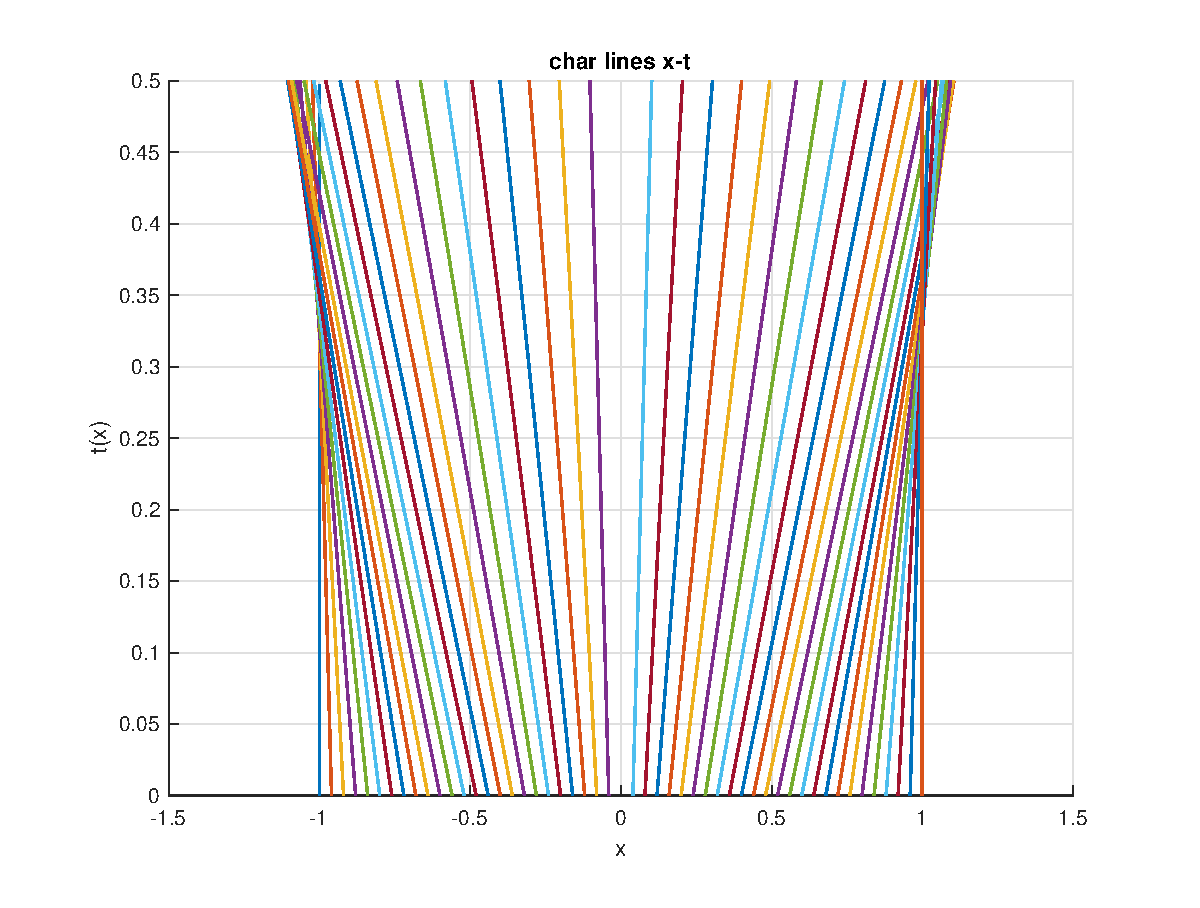
\includegraphics[width=10cm]{xt_char.eps}
\centering
\caption{char curves in the $x-t$ plane}
\end{figure}



\subsubsection{solution $u$ at three times}
At $t = 0$, the solution is simply the initial data:
$$
	u(x,0) = sin(\pi x)
$$
\newpage
\begin{figure}[t]
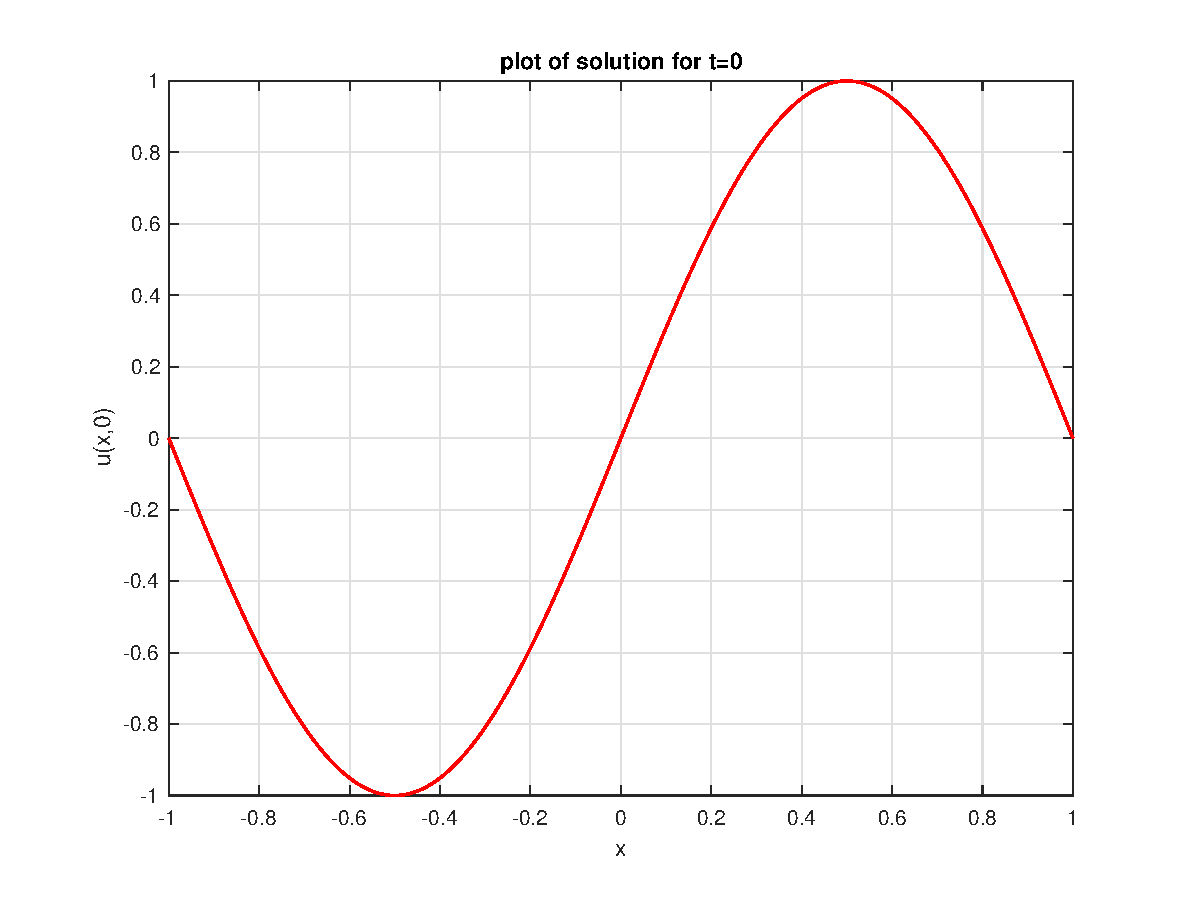
\includegraphics[width=10cm]{bur_t1.eps}
\centering
\caption{solution $u$ at time $t = 0$}
\end{figure}

At other times, we use the implicit solution given above:
$$
	u(x,t) = sin(\pi(x-ut))
$$ and plot the solution.

At $t = 0.25$, we have:
$$
	u(x,0.25) = sin(\pi(x-0.25u))
$$
\newpage 
\begin{figure}[t]
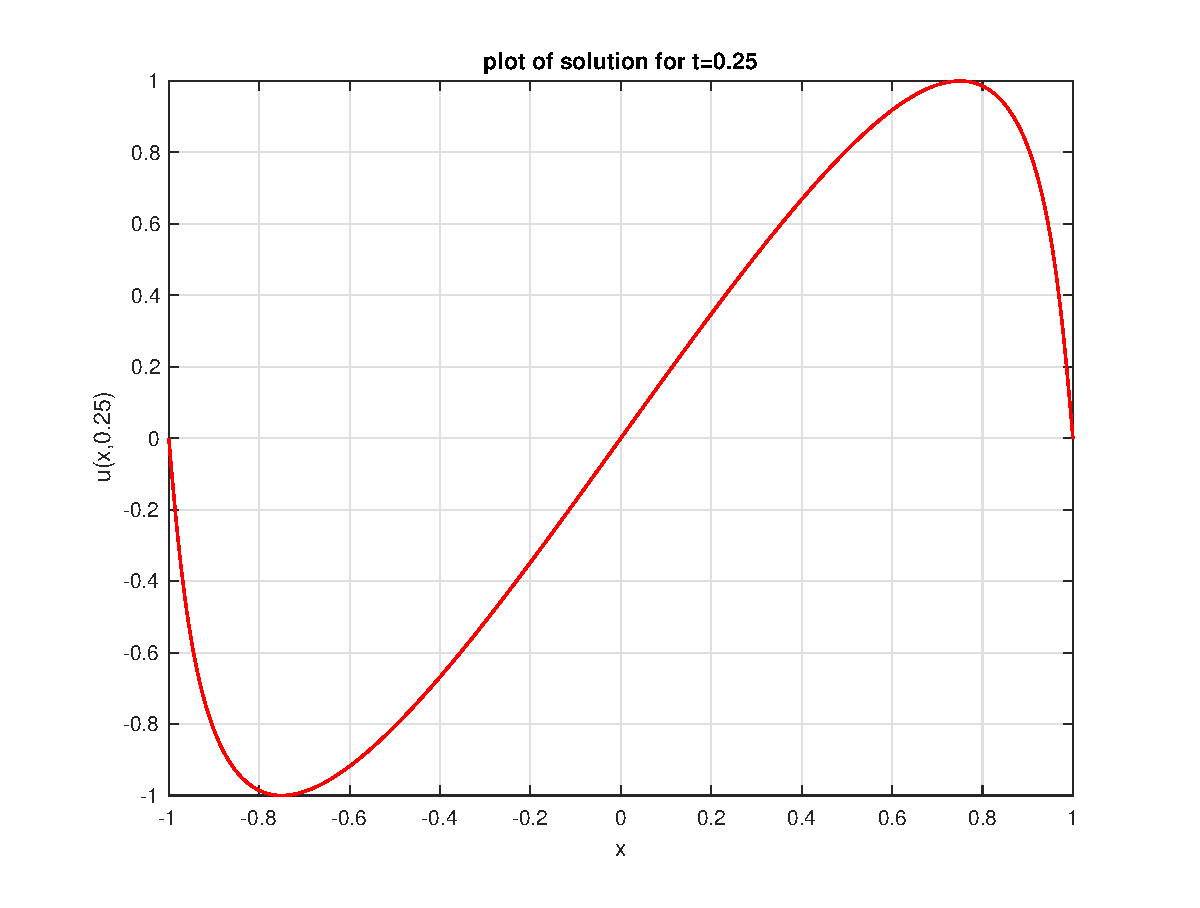
\includegraphics[width=10cm]{u_25.eps}
\centering
\caption{solution $u$ at time $t = 0.25$}
\end{figure}

At $t = 0.5$, we have:
$$
	u(x,0.5) = sin(\pi(x-0.5u))
$$
\newpage 

\begin{figure}[t]
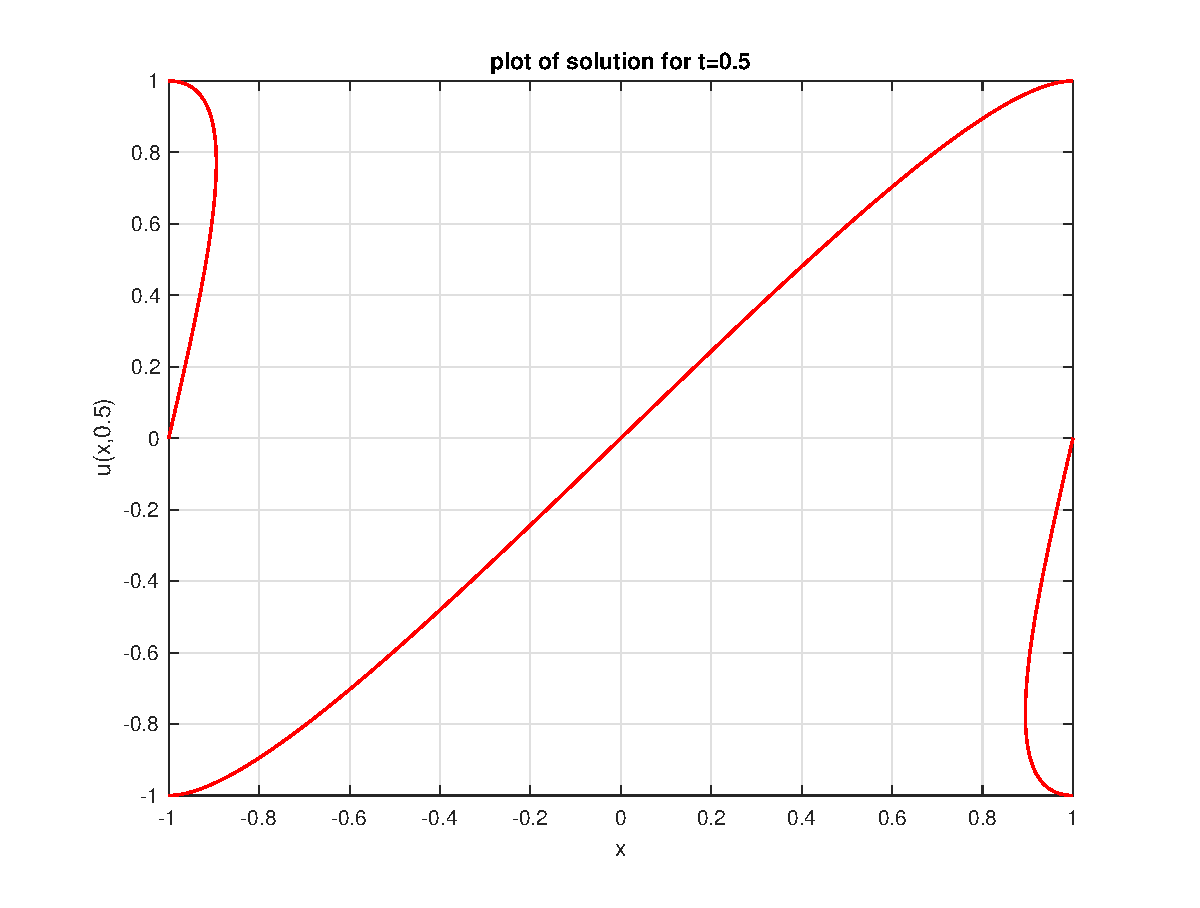
\includegraphics[width=10cm]{u_5.eps}
\centering
\caption{solution $u$ at time $t = 0.5$}
\end{figure}

\newpage
For clarity, we extend $x$ to $\big[-1.5,1.5\big]$ and observe the wave.

\begin{figure}[t]
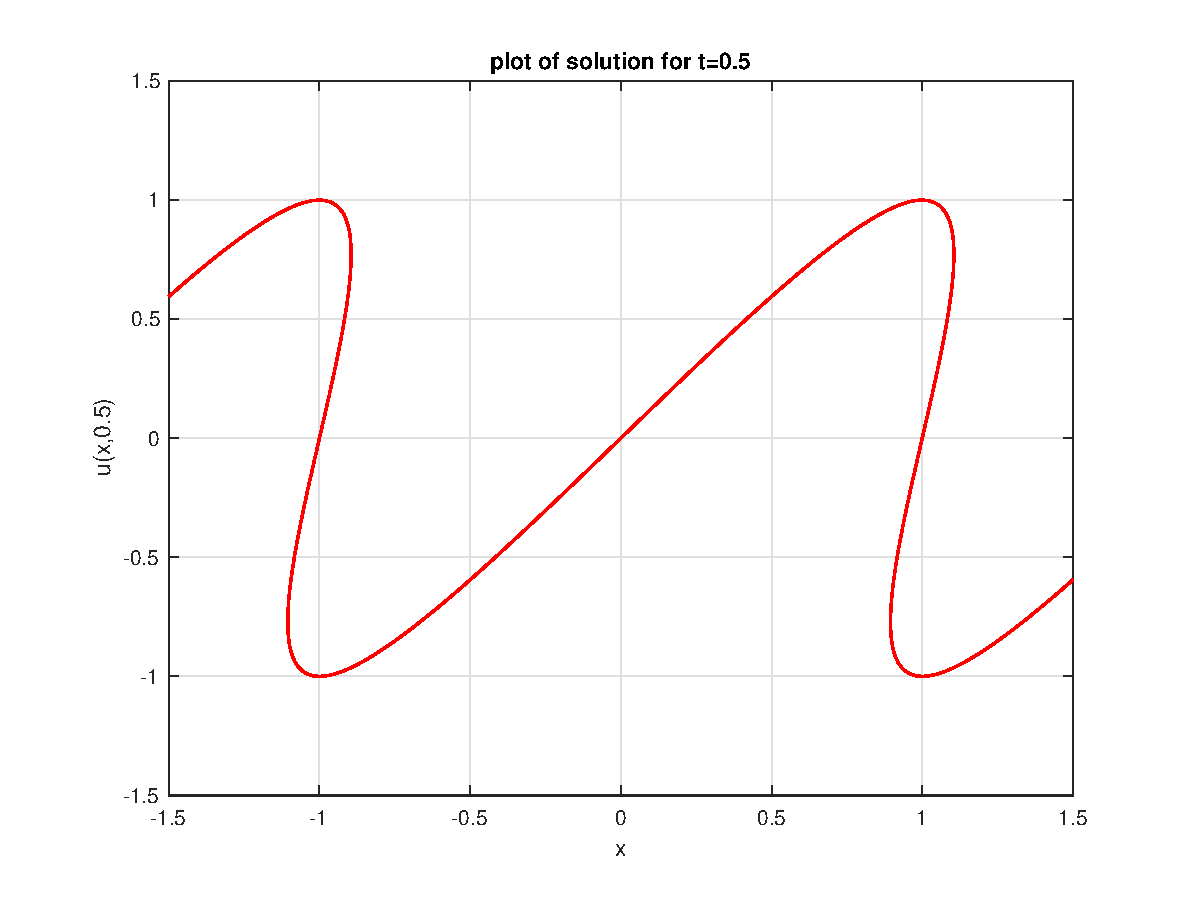
\includegraphics[width=10cm]{e_5_2.eps}
\centering
\caption{solution $u$ at time $t = 0.5$, extended for illustration}
\end{figure}



\newpage
\subsection{Weak formulation of the problem}
Let $V_h\in \{v\in L^2(K): v\rvert_{K}\in \mathbb{P}^1(K), \forall K \in T_K\}$ be the functional space for our Galerkin formulation. We take an arbitrary test function $v\in V_h$ multiplied on both sides of:
$$
	\pdx{t}u + \pdx{x}f(u) = 0
$$ here $f(u) = \frac12 u^2$ is the flux term.
$$
	\pdx{t} u\cdot v + \pdx{x}f(u) \cdot v = 0
$$ and integrate on each element:
$$
	\int_{K}\pdx{t}u\cdot v dx+ \int_{K}\pdx{x}f(u)\cdot vdx = 0
$$

Then the weak form becomes: find $u_h\in V_h$ such that
$$
	\int_{K}\pdx{t}u_h\cdot vdx + \int_{K}\pdx{x}f(u_h)\cdot vdx = 0
$$ for all $v\in V_h$, where $f(u) = \frac12 u^2$.

We replace $v$ with a basis function $\phi_j^K$ defined on each individual element $K \in T_K$, we have:
$$
	\int_{K}\pdx{t}u_h \cdot \phi_j^K dx + \int_{K}\pdx{x}f(u_h)\cdot \phi_j^Kdx = 0
$$ $\forall \phi_j^K\in V_h$.

Since we are in 1D, each $K$ is an interval, we can integrate by parts to get to the semi-discrete formulation:
$$
	\int_{K}\pdx{t}u_h\phi_j^Kdx + \bigg[f(u_h)\cdot\phi_j^K\bigg]\bigg\rvert_K - \int_Kf(u_h)\cdot\pdx{x}\phi_j^Kdx  = 0
$$
\subsection{Matrix form of the semi-discrete problem}
To get the matrix form, we use $u_h = \sum_{i=0}^{p}u_i^K\phi_i^K$, where $p$ is the polynomial degree of element functions. Along with the nodal basis expansion of $f$ since $f(u_h)$ is nonlinear, we have:
$$
	f(u_h) = \sum_{i=0}^{p}f_{i}^K\phi_i^K
$$

In summary:
$$
	u_h(x,t) = \sum_{i=0}^pu_i^K(t)\phi_i^K(x)
$$
$$
	f(u_h)(x,t) = \sum_{i=0}^pf_i^K(t)\phi_i^K(x)
$$ and there is no source term.

We also need to define:
$$
	\bigg[f(u_h)\cdot\phi_j^K\bigg]\bigg\rvert_K 
$$ at the cell interfaces. By introducing the numerical flux $\hat{F}(u_L,u_R)$, we have:
$$
	\bigg[f(u_h)\cdot\phi_j^K\bigg]\bigg\rvert_K = 
	\bigg[\hat{F}(u_L,u_R)\bigg](x_K)\phi_j^K(x_K) - 
	\bigg[\hat{F}(u_L,u_R)\bigg](x_{K-1})\phi_j^K(x_{K-1})
$$

We plug the expansions into the original semi-discrete form:
$$
	\sum_{i=0}^p\pdx{t}u_i^K\int_{K}\phi_i^K\phi_j^Kdx
	- \sum_{i=0}^pf_{i}^K\int_{K}\phi_i^K\pdx{x}\phi_j^Kdx
$$
$$
	= - \bigg[\hat{F}(u_L,u_R)(x_K)\phi_j^K(x_K) - \hat{F}(u_L,u_R)(x_{K-1})\phi_j^K(x_{K-1})\bigg]
$$

We use this general formulation and apply on our Burger's equation. Here we use linear functional elements, and use a Lax-Friedrichs numerical flux function. $f(u_h) = \frac12 u_h^2$:
$$
	u_h^K = \sum_{i=0}^1u_{i}^K\phi_i^K
$$
$$
	f(u_h^K)= \frac12\sum_{i=0}^1(u_i^K)^2\phi_i^K
$$ here $u_i^K = u^K(x_i,t)$ is the value of $u_h$ at $(x_i, t)$.

Then we can write out the matrix form as:
\begin{equation}\label{eqn:matform}
	M^K\mathbf{\dot{u_h}^K} - (C^K)^T\mathbf{f_{h}^K} =
	-\bigg[\phi^K(x)\hat{F}(u_L,u_R)(x)\bigg]\bigg\rvert_K
\end{equation} where $M$ is the mass matrix, $M_{ij}^K = \int_{K}\phi_i(x)\phi_j(x)dx$, $C_{ij}^K = \int_{K}\phi_i(x)\pdx{x}\phi_j(x)dx$. $u_h^K,f_h^K$ are vectors of form:
$$
	u_h^K = 
	\begin{pmatrix}
		u_0^K \\
		u_1^K
	\end{pmatrix}
$$
$$
	f_h^K =
	\begin{pmatrix}
		\frac12(u_0^K)^2 \\
		\frac12(u_1^K)^2
	\end{pmatrix}
$$

Our basis functions are linear, in 1D, define:
$$
	\phi_{i}^K(x) = a_ix+b_i
$$

For each element $K$, we have 2 basis functions, $\{\phi_0^K, \phi_1^K\}$. In our problem, we have:
$$
\begin{cases}
	K_1 = \big[-1,-\frac12\big]\\
	K_2 = \big[-\frac12,0\big]\\
	K_3 = \big[0,\frac12\big]\\
	K_4 = \big[\frac12,1\big]
\end{cases}
$$

For each element $K_i$, $i =1,2,3,4$, we define the linear bases as follows:
$$
\begin{cases}
	\phi_0^{K_i}(x_{k-1}) = 1 \\
	\phi_0^{K_i}(x_{k}) = 0
\end{cases}
$$

$$
\begin{cases}
	\phi_1^{K_i}(x_{k-1}) = 0 \\
	\phi_1^{K_i}(x_{k}) = 1
\end{cases}
$$

Using this constraint, we calculate the 8 basis functions:
$$
	K_1 = \big[-1,-\frac12\big]
	\begin{cases}
		\phi_0^{K_1}(x) = -2x-1 \\
		\phi_1^{K_1}(x) = 2x+2
	\end{cases}
$$
$$
	K_2 = \big[-1/2,0\big]
	\begin{cases}
		\phi_0^{K_2}(x) = -2x \\
		\phi_1^{K_2}(x) = 2x+1
	\end{cases}
$$
$$
	K_3 = \big[0,1/2\big]
	\begin{cases}
		\phi_0^{K_3}(x) = -2x+1\\
		\phi_1^{K_3}(x) = 2x
	\end{cases}
$$
$$
	K_4 = \big[1/2,1\big]
	\begin{cases}
		\phi_0^{K_4}(x) = -2x+2\\
		\phi_1^{K_4}(x) = 2x-1
	\end{cases}
$$

The linear bases are as follows:
\newpage
\begin{figure}[t]
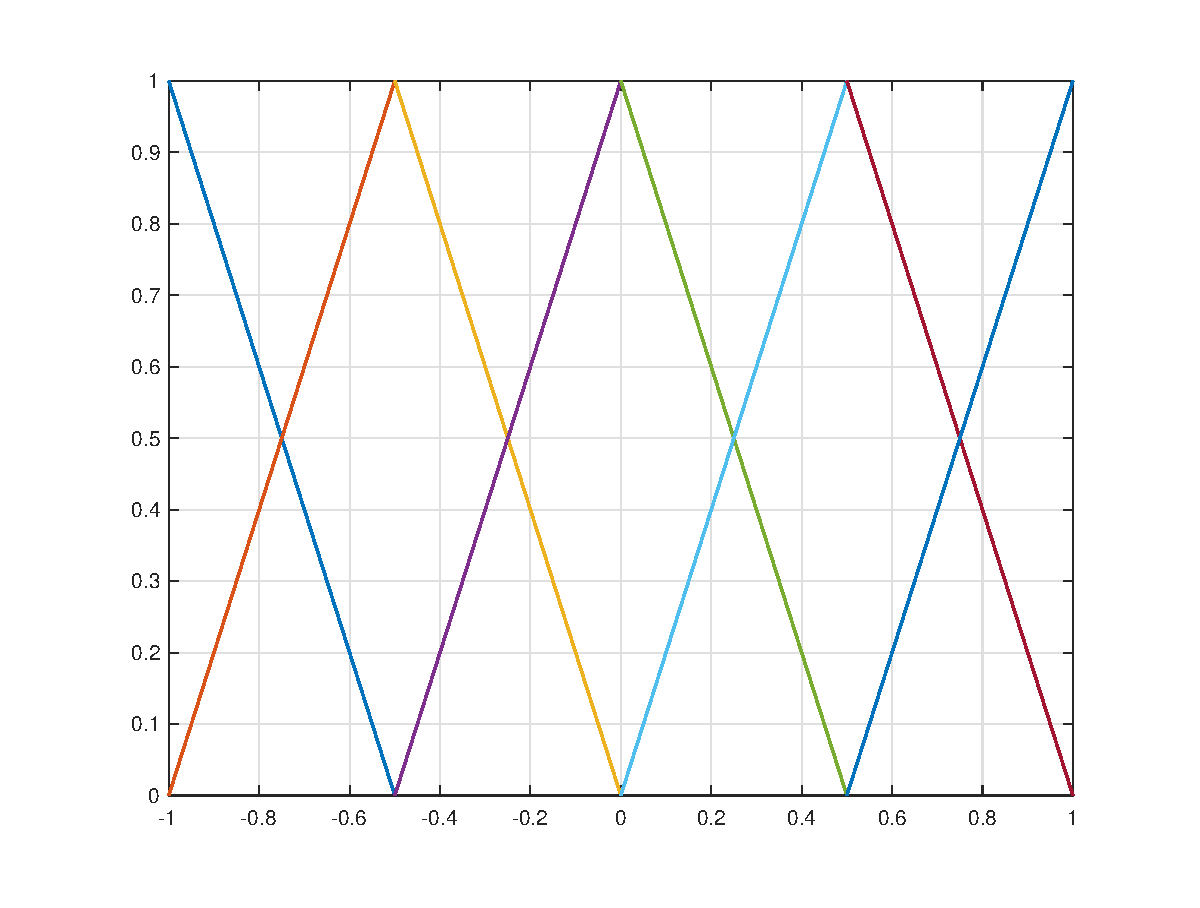
\includegraphics[width=10cm]{linear_basis.eps}
\centering
\caption{8 linear basis functions on $\{K_1,K_2,K_3,K_4\}$}
\end{figure}

Knowing the $\phi$ basis functions, we will be able to calculate the matrix entries, in the following:

For each element $K_i, i=1,2,3,4$, we need to solve a matrix equation of form \ref{eqn:matform}. We calculate each equation since we have all the tools:

Using MATLAB symbolic computation with the above 8 basis functions, we compute:
$$
	M^{K_i} = 
	\begin{pmatrix}
		\frac16 & \frac{1}{12}\\
		\frac{1}{12} & \frac16
	\end{pmatrix}
$$ 
$$
	C^{K_i} = 
	\begin{pmatrix}
		-\frac12 & \frac{1}{2}\\
		-\frac{1}{2} & \frac12
	\end{pmatrix}
$$

for all $i = 1,2,3,4$.

Then we have a system of ODEs:
$$
	\frac{d}{dt}
	\begin{pmatrix}
		u_0^K \\
		u_1^K
	\end{pmatrix} =
	\frac12(M^K)^{-1}\cdot(C^K)^T 
	\begin{pmatrix}
		\big(u_0^K\big)^2 \\
		\big(u_1^K\big)^2
	\end{pmatrix}
	-
	(M^K)^{-1}
	\begin{pmatrix}
		-\big[\hat{F}(u_L,u_R)\big](x_{k-1}) \\
		\big[\hat{F}(u_L,u_R)\big](x_{k})
	\end{pmatrix}
$$
$$
	= \mathcal{F}(u_0^K, u_1^K)
$$

For numerical flux, we have:
$$
	\bigg[\hat{F}(u_L, u_R)\bigg]
	=
	\frac12\bigg[f(u_L) +f(u_R)\bigg]+\frac{c}{2}(u_L-u_R)
$$

For the last flux vector, we calculate:
At $x_{k-1}$
$$
	\big[\hat{F}(u_L,u_R)\big]_{x_{k-1}}
	=
	\frac12\big(f(u_{1}^{K-1})+f(u_{0}^{K})\big) + \frac12c\big(u_1^{K-1} - u_0^K\big)
$$
$$
	= \frac12\big(\frac12(u_{1}^{K-1})^2+\frac12(u_{0}^{K})^2\big) + \frac12c\big(u_1^{K-1} - u_0^K\big)
$$
$$
	= \frac14((u_{1}^{K-1})^2 + (u_{0}^{K})^2) + \frac12c\big(u_1^{K-1} - u_0^K\big)
$$

Similarly at $x_k$:
$$
	\big[\hat{F}(u_L,u_R)\big]_{x_{k}}
	=
	\frac14((u_{1}^{K})^2 + (u_{0}^{K+1})^2) + \frac12c\big(u_1^{K} - u_0^{K+1}\big)
$$

Here we have a few choices for the constant $c$, one possibility is:
$$
	c\ge \max_{\inf u_h(x)\le s\le \sup u_h(x)}f_u(s)
$$

Here we have $f_u = (\frac{1}{2}u^2)' = u$, and with the sine initial condition, we know that $u$ will never exceed 1 $(\abs{u_h(x)}\le 1)$. Then $c = 1$ would be a good choice. 

To be more clear, we can arrange the entire triangulation of $V_h$ into a global matrix. Since elements do not share continuities, we can directly "stack" them in the matrix, we finally obtain:
$$
	\frac{d}{dt} 
	\begin{pmatrix}
		u_0^1 \\
		u_1^1 \\
		\vdots \\
		u_0^4 \\
		u_1^4 \\
	\end{pmatrix} 
	= \frac12 \hat{M}\hat{C} \cdot
	\begin{pmatrix}
		(u_0^1)^2 \\
		(u_1^1)^2 \\
		\vdots \\
		(u_0^4)^2 \\
		(u_1^4)^2
	\end{pmatrix} +
	\hat{M}
	\begin{pmatrix}
		\big[\hat{F}(u_0^1, u_1^0)\big] \\
		-\big[\hat{F}(u_0^2, u_1^1)\big] \\
		\vdots \\
		\big[\hat{F}(u_0^4, u_1^3)\big] \\
		-\big[\hat{F}(u_0^5, u_1^4)\big] \\
	\end{pmatrix}
$$ where:
\[M =  \begin{pmatrix} (M^1)^{-1} & & & \\  &(M^2)^{-1}  & & \\ & & (M^3)^{-1} & \\  & & & (M^4)^{-1}  \end{pmatrix} \] and
\[C = \ \begin{pmatrix} (C^1)^T & & & \\  &(C^2)^T & & \\ & & (C^3)^T& \\  & & & (C^4)^T\end{pmatrix}.\]

Then the final forward Euler discrete form is as follows:
\begin{eqnarray}
	\begin{pmatrix}
		u_0^1 \\
		u_1^1 \\ 
		\vdots \\
		u_0^4 \\
		u_1^4 \\ 
	\end{pmatrix}(t_{m+1}) =
		\begin{pmatrix}
		u_0^1 \\
		u_1^1 \\ 
		\vdots \\
		u_0^4 \\
		u_1^4 \\ 
	\end{pmatrix}(t_{m})  + 
	\Delta t\left(\frac{1}{2} \hat{M}\hat{C}
	\begin{pmatrix}
		\big(u_0^1\big)^2 \\
		\big(u_1^1\big)^2 \\
		\vdots \\
		\big(u_0^4\big)^2 \\
		\big(u_1^4\big)^2 \\
	\end{pmatrix} (t_m)
	+
	\hat{M}
	\begin{pmatrix}
 - F(u_0^{1}, u_1^{0}) \\ F(u_0^{2}, u_1^{1}) \\ \vdots \\  - F(u_0^{4}, u_1^{3}) \\ F(u_0^{5}, u_1^{4})
	\end{pmatrix}(t_m)\right)
\end{eqnarray} with appropriate choices of $\Delta t, \Delta x$ considering the CFL condition.

We present the numerical solutions in the sections that follow.



\section{Numerical Burger's Equation MATLAB Program Experiments: Linear Basis}

\indent \indent After implementing the Lax-Friedrichs step for the weak form, we can present the numerical solutions with number of elements $N = 4, 10, 20, 50$. We first present the entire evolution with the best discretization with $N = 50$:
\newpage

\begin{figure}[t]
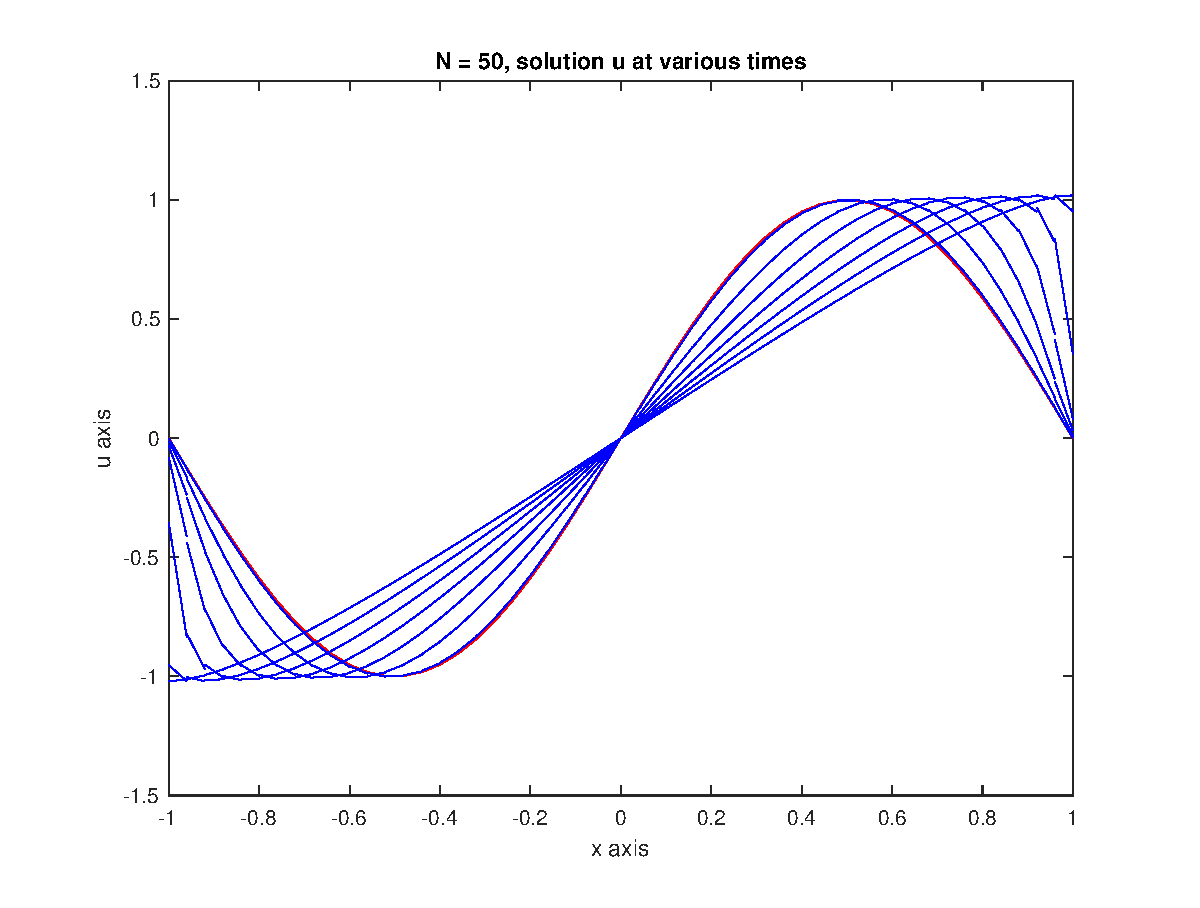
\includegraphics[width=10cm]{p2best.eps}
\centering
\caption{Full solution evolution using $N = 50$, for illustration}
\end{figure}

We see we have obtained accurate numerical solutions that capture the wave. We present the different plots obtained from different $N$'s, for the plots below, the blue line is always $t = 0$, then purple line is $t = 0.25$, black line is $t = 0.5$.

\subsection{Solutions using $N = 4$}
\indent \indent Using $N=4$ linear elements, we overlay the numerical solutions at time $t = 0, t = 0.25, t = 0.5$, presented below:
\newpage
\begin{figure}[t]
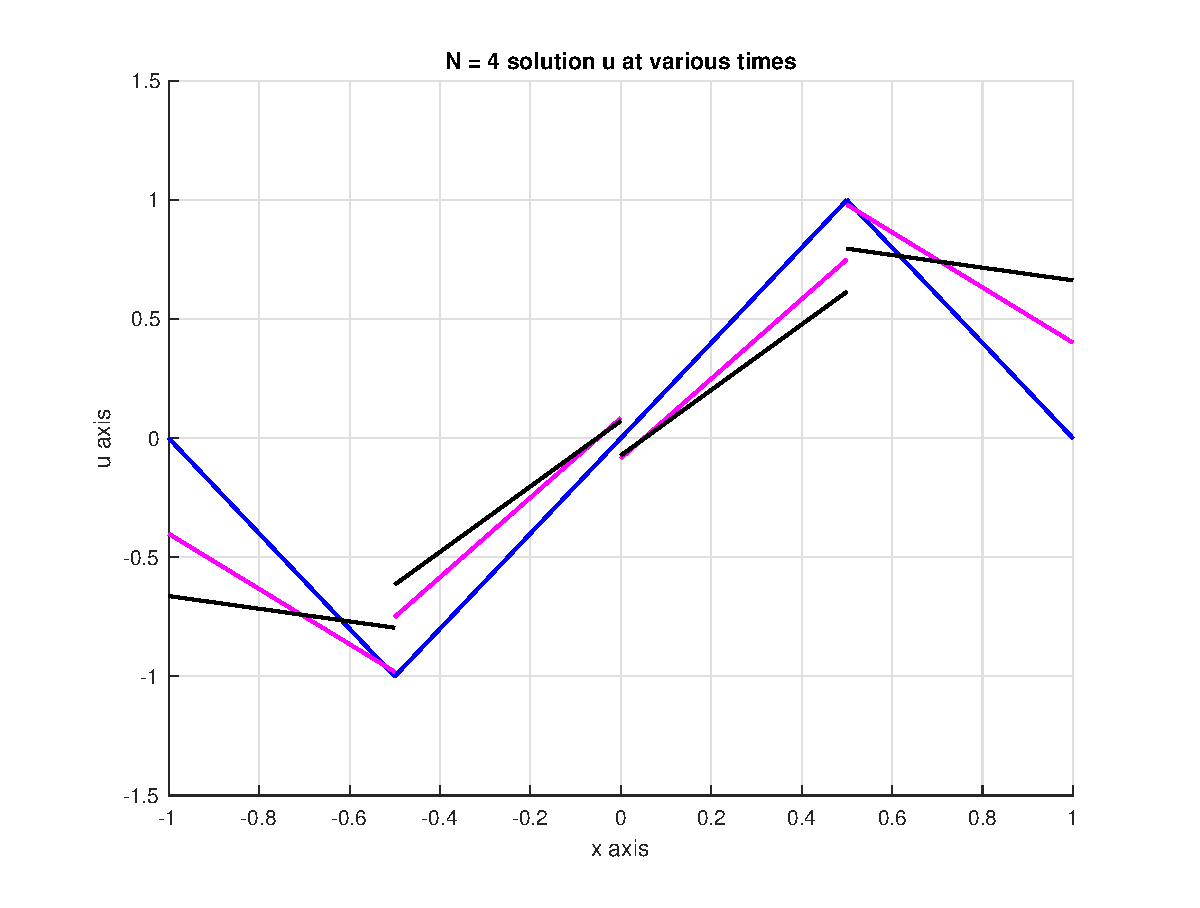
\includegraphics[width=10cm]{overlayn4.eps}
\centering
\caption{Linear DG with $N=4$}
\end{figure}
\newpage

\subsection{Solutions using $N=10$}
\newpage
\begin{figure}[t]
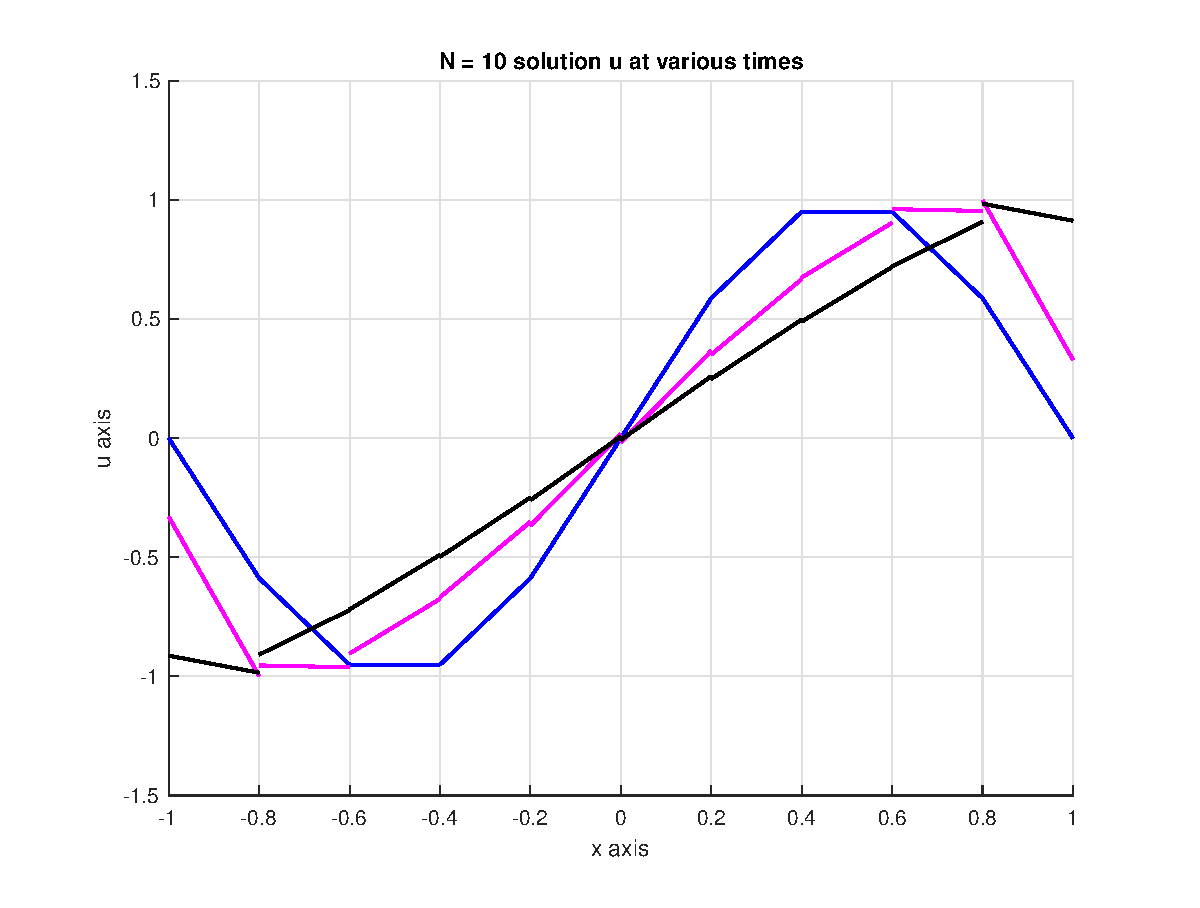
\includegraphics[width=10cm]{overlayn10.eps}
\centering
\caption{Linear DG with $N=10$}
\end{figure}
\newpage

\subsection{Solutions using $N=20$}
\newpage
\begin{figure}[t]
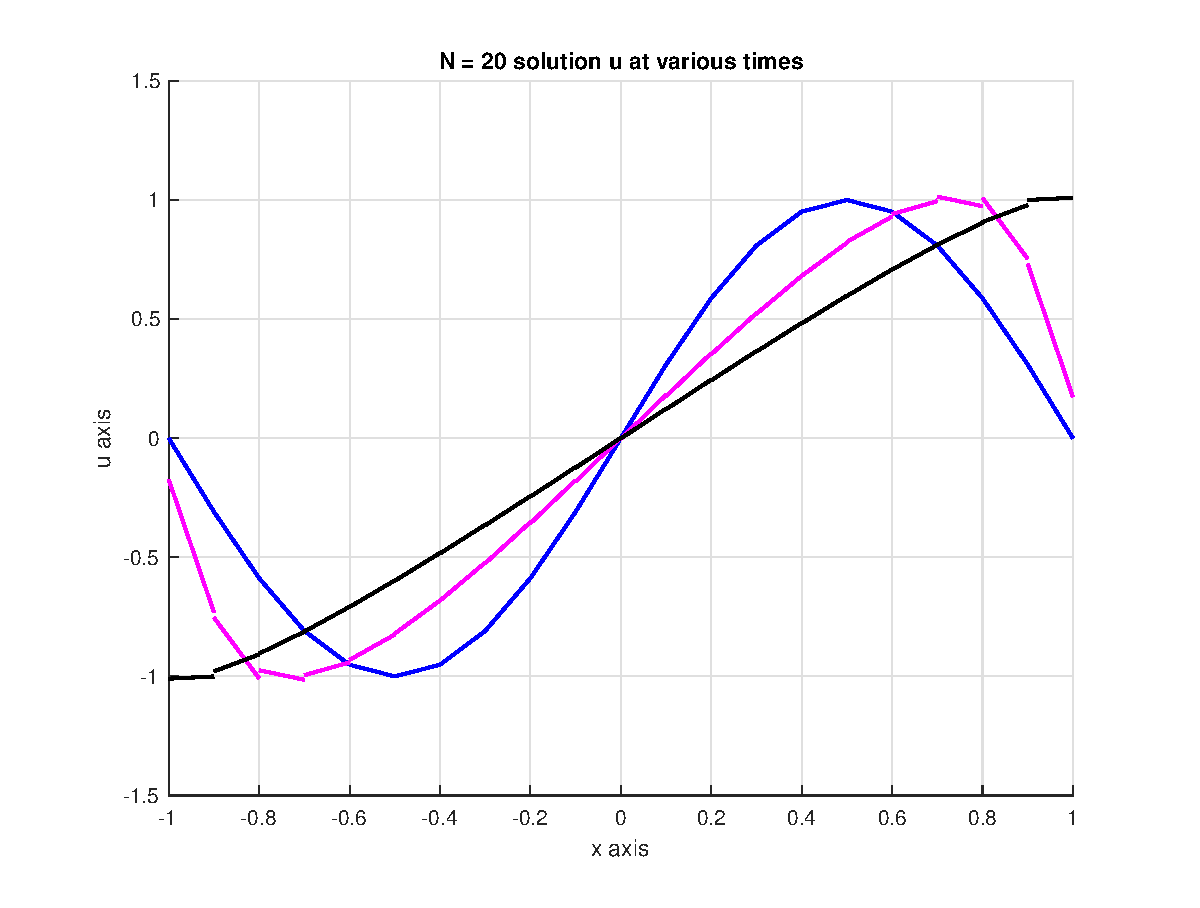
\includegraphics[width=10cm]{overlayn20.eps}
\centering
\caption{Linear DG with $N=20$}
\end{figure}
\newpage


\subsection{Solutions using $N=50$}
\newpage
\begin{figure}[t]
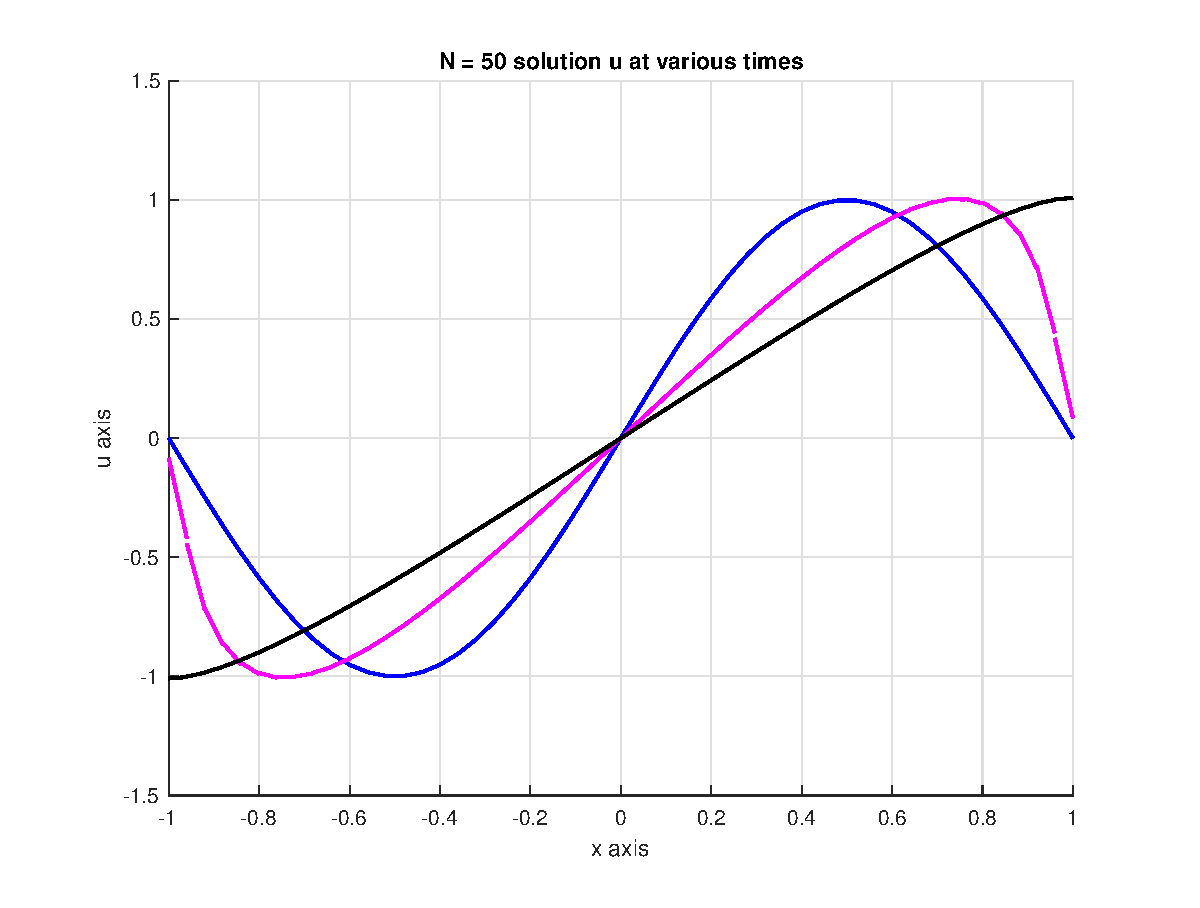
\includegraphics[width=10cm]{overlayn50.eps}
\centering
\caption{Linear DG with $N=50$}
\end{figure}
\newpage

\subsection{comment on refined mesh and observations}
\indent \indent We first note that the linear elements are discontinuous at cell interfaces, see the mismatched cell interfaces especially when $N$ is small; we see this is a feature of DG methods, since we do not impose continuity requirements, we can have jump discontinuities for the linear elements. As we refine $N$, the solution becomes more and more smooth and we are able to capture the wave behavior. In the limit as $N\rightarrow\infty$, the numerical solution does converge to the true solution and the discontinuities would be negligible.


\section{Numerical Burger's Equation MATLAB Program Experiments: Lagrange Basis}
\subsection{numerical solution with $P=3$, $N = 20$ at two times $t = 0.25$ and $t = 0.5$}
\indent \indent In this plot, the colored line is the initial condition, the blue line is the solution at $t = 0.25$, the black line is the solution $t = 0.5$.
\newpage
\begin{figure}[t]
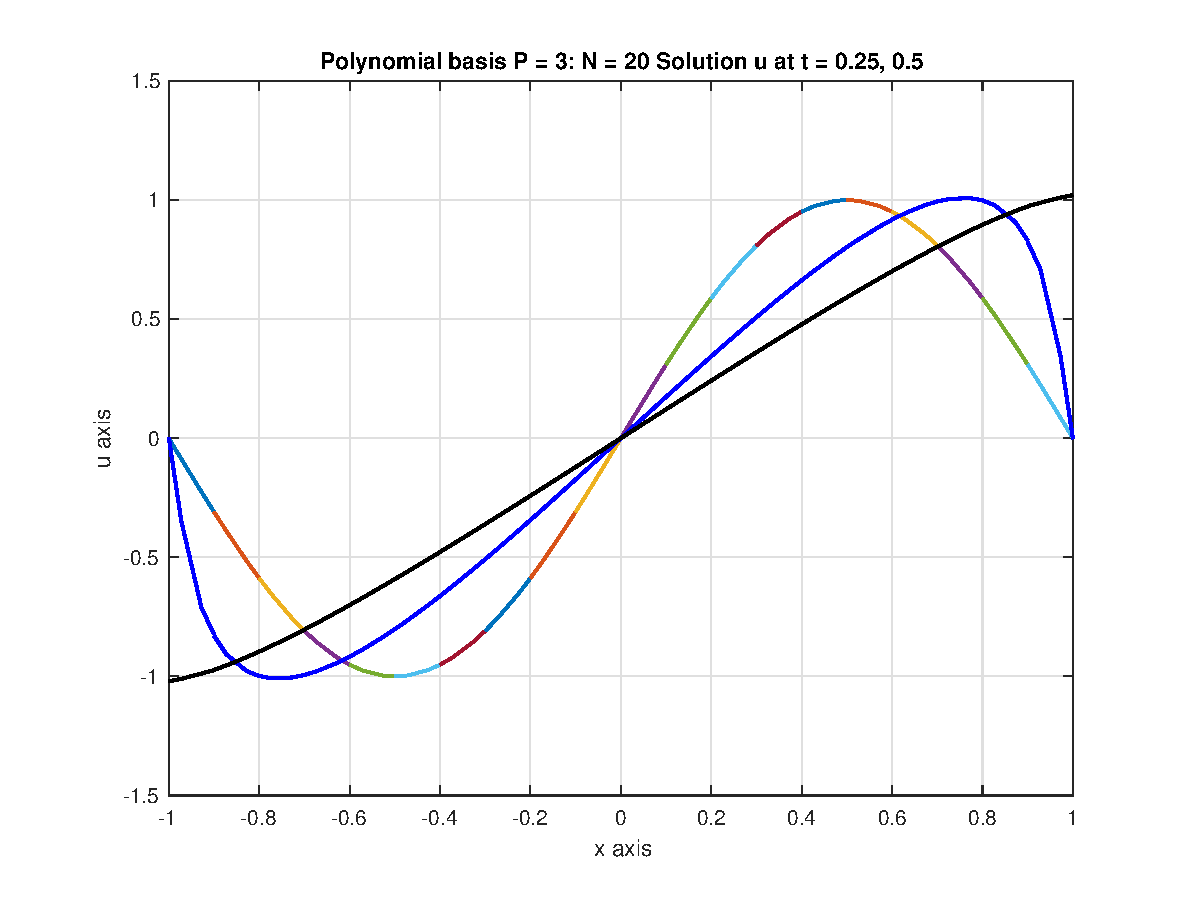
\includegraphics[width=10cm]{p3a.eps}
\centering
\caption{Cubic DG with $N=20$, at $t = 0.25, 0.5$}
\end{figure}
\newpage

\subsection{numerical solution with $P = 1$, $N = 20$ at two times $t = 0.25$ and $t = 0.5$}
In comparison, we use the same conditions, but instead use linear elements, the plot is presented below. The colored line is initial condition, the blue line is solution at $t = 0.25$, the black line is solution at $t = 0.5$.
\newpage
\begin{figure}[t]
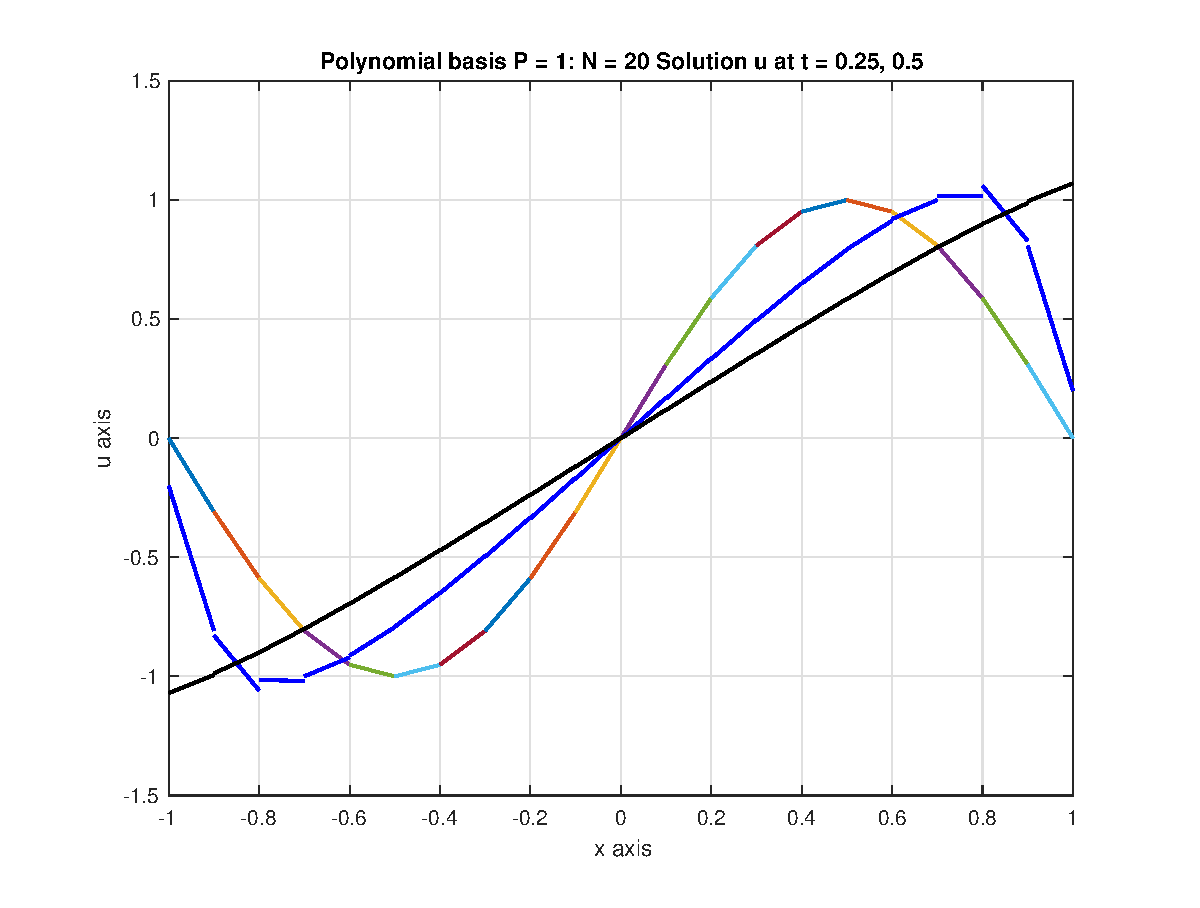
\includegraphics[width=10cm]{p3b.eps}
\centering
\caption{Linear DG with $N=20$, at $t=0.25,0.5$}
\end{figure}
\newpage


\subsection{numerical solution with $P = 1$, $N = 50$ at two times $t = 0.25$ and $t = 0.5$}
\newpage
Lastly we plot the linear elements with $N = 50$.
\begin{figure}[t]
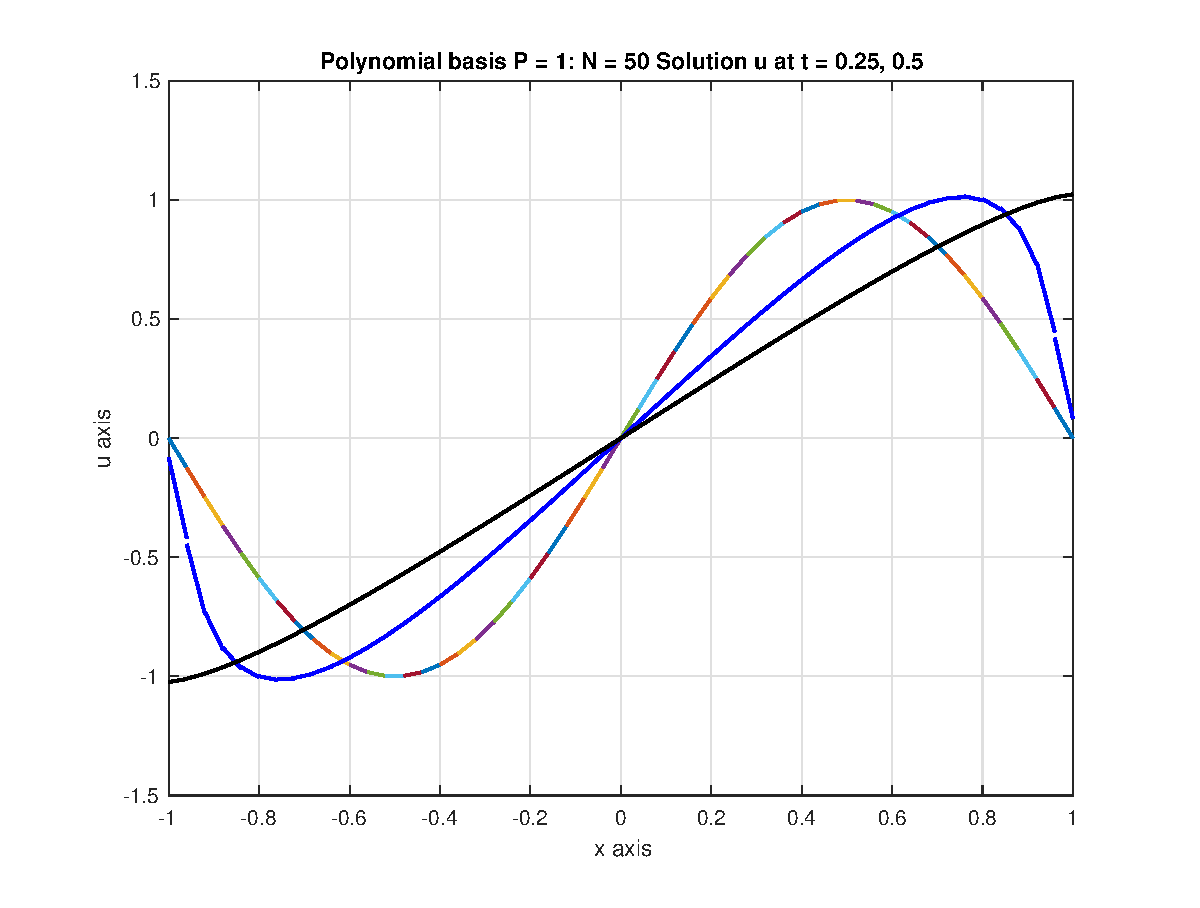
\includegraphics[width=10cm]{p3c.eps}
\centering
\caption{Linear DG with $N=50$, at $t = 0.25,0.5$}
\end{figure}


\subsection{Overlaid Comparison and Comments}
We overlay the results from part 1, 2, and 3 at two times $t = 0.25$, $t = 0.5$, and label the approaches.
\newpage
\begin{figure}[t]
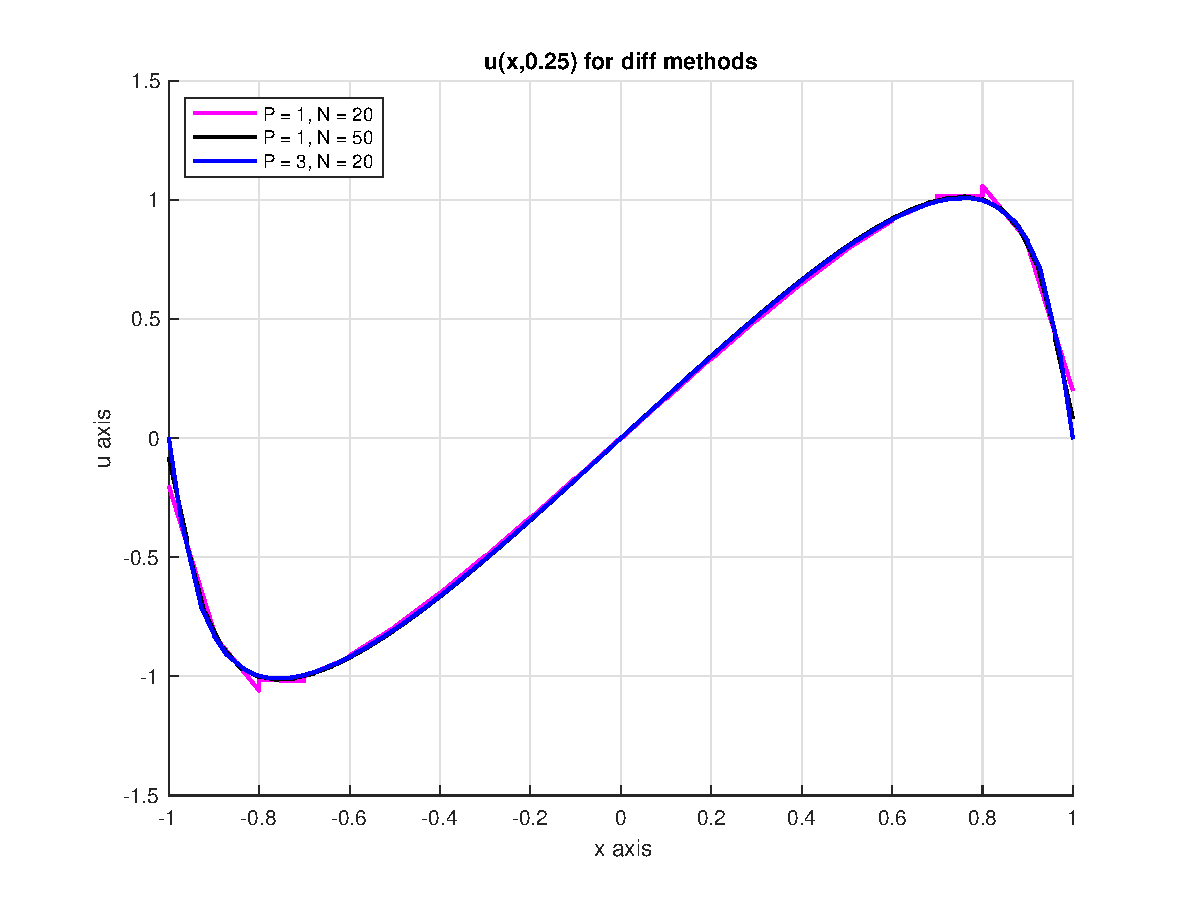
\includegraphics[width=10cm]{p3cp25.eps}
\centering
\caption{numerical solution for $t = 0.25$ for 3 methods, labelled}
\end{figure}

In order to better illustrate the 3 curves, we zoom in and observe their differences.

\begin{figure}[t]
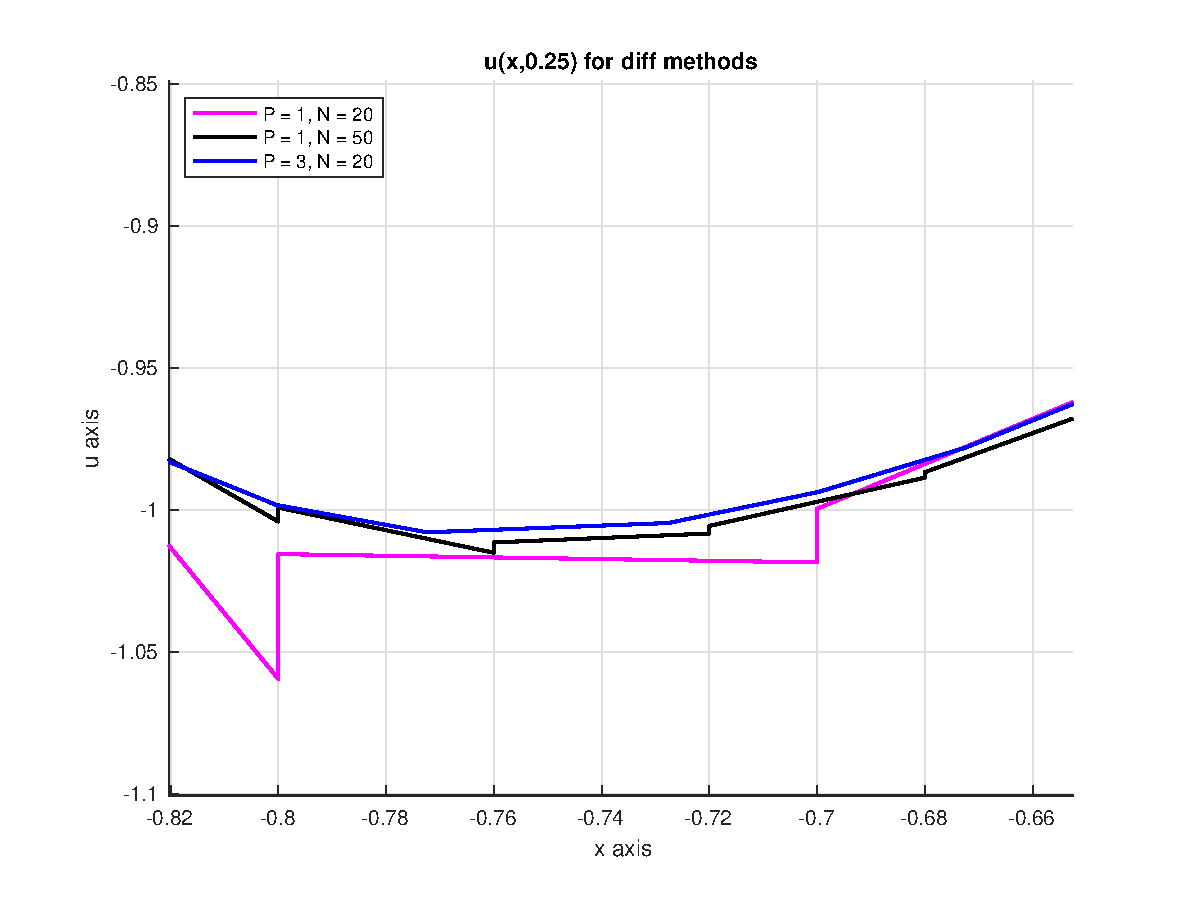
\includegraphics[width=10cm]{zoom1.eps}
\centering
\caption{local numerical solutions using 3 methods, $t = 0.25$}
\end{figure}

\newpage
We do the same for $t = 0.5$, and zoom in to illustrate the differences better.
\newpage
\begin{figure}[t]
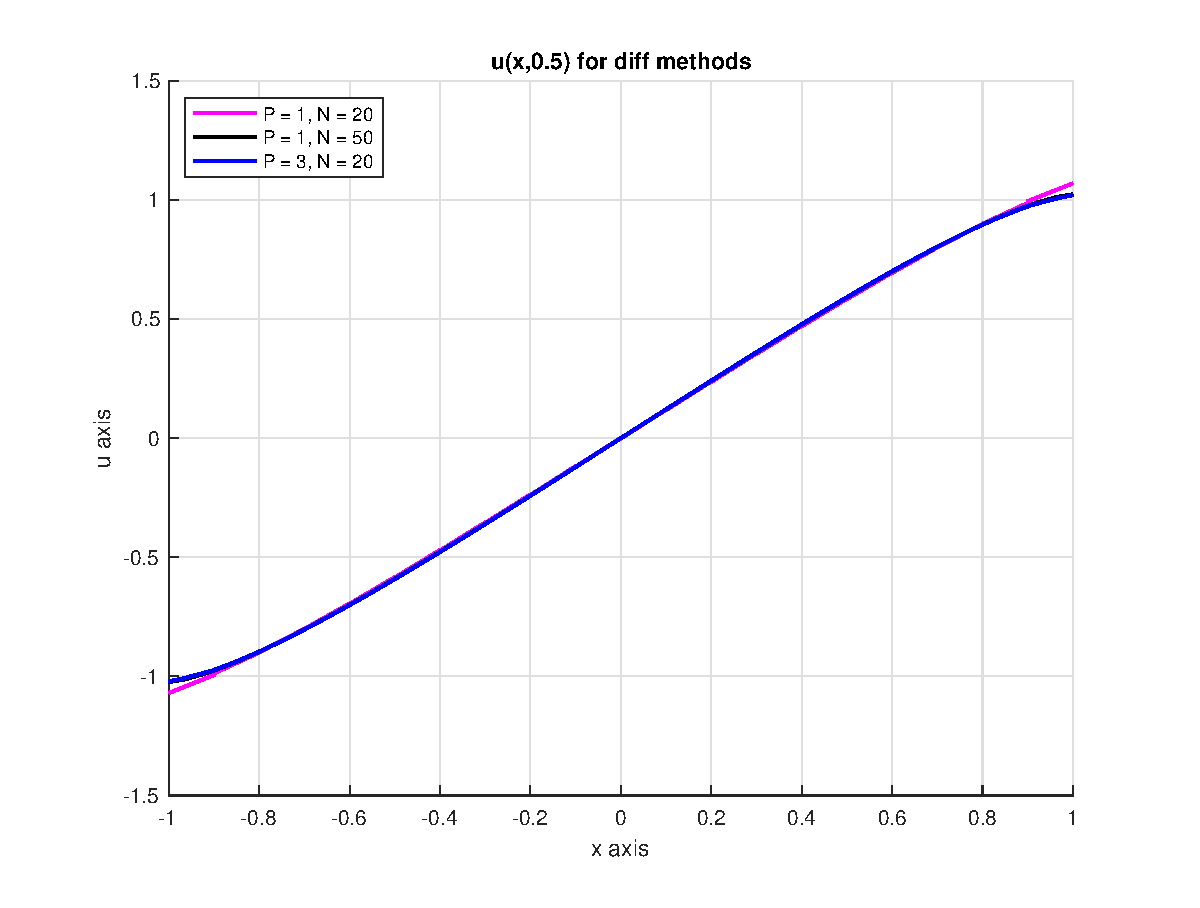
\includegraphics[width=10cm]{p3cp5.eps}
\centering
\caption{numerical solution for $t = 0.5$ for 3 methods, labelled}
\end{figure}

We zoom in, at around the same location as $t = 0.25$ in the previous plot.
\newpage
\begin{figure}[t]
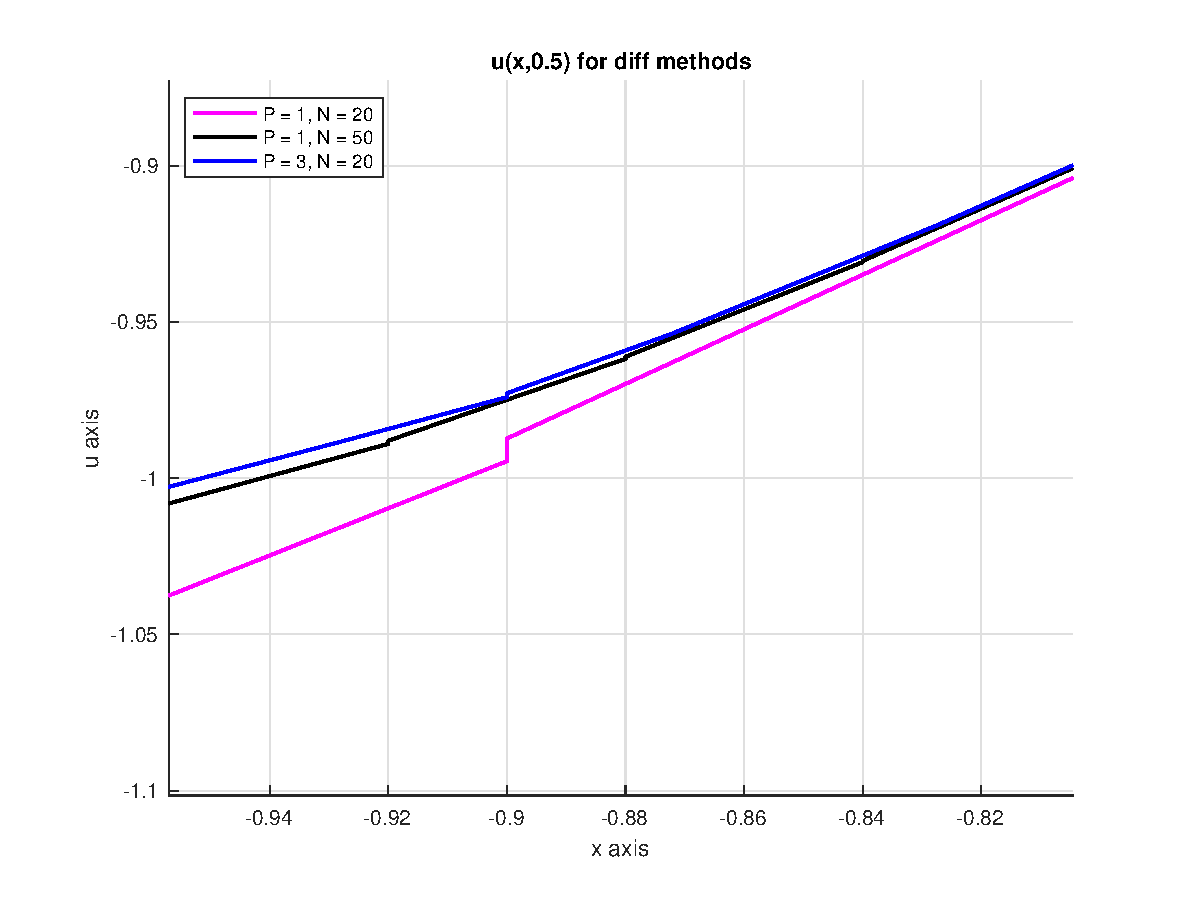
\includegraphics[width=10cm]{zoom2.eps}
\centering
\caption{local numerical solutions using 3 methods, $t = 0.5$}
\end{figure}

\newpage
We make the observation that cubic elements are naturally smoother than linear elements (as expected in the plots, we have fewer discontinuities/jumps). Since the polynomial is higher order, we are able to obtain a relatively satisfactory approximation to the true solution even with fewer elements. As shown in the zoomed-in graph, it takes 50 elements versus 20 elements, for linear elements to perform nearly as good as cubic elements. If higher computational cost associated with computing the Legendre bases is permissible, we would certainly use higher order polynomials since they offer much better convergence for even fewer elements. Nonetheless, all discretization and methods are able to capture the wave advection.

% ================ end file
\end{document}

